\section{Model Description}

The Simple Navigation model in the AVS Basilisk simulation is used to generate 
a stand-in for the real navigation system.  Its use-case is to provide realistic 
navigation signals that are right at the spec of what ADCS claims for navigation 
system performance.  For a typical spacecraft navigation system, the spec will 
almost always be at least a factor of two lower in performance than the expected 
nominal capabilities of the on-board navigation system.  Therefore, we require 
the existence of a model that can provide spec-level navigation errors so that 
the functionality of the guidance and control subsystems can be verified as 
acceptable in the presence of navigation errors that are right at the spec. \\

The noise present in the simple navigation is designed to mimic the error signals 
that will be observed in the real navigation system.  The true "noise" present 
in a vehicle's navigation system is always a combination of bias, white noise, 
and brown noise (or random walk).  In order to provide this, a second-order 
Gauss-Markov process model was added to the simulation utilities that allows 
the user to configure a random walk process.  The output of this model when 
applied to the vehicle position can be observed in Figure~\ref{fig:SimpleNavPos}, 
and the attitude can be observed in Figure~\ref{fig:SimpleNavAtt}.

\begin{figure}[htbp]\centerline{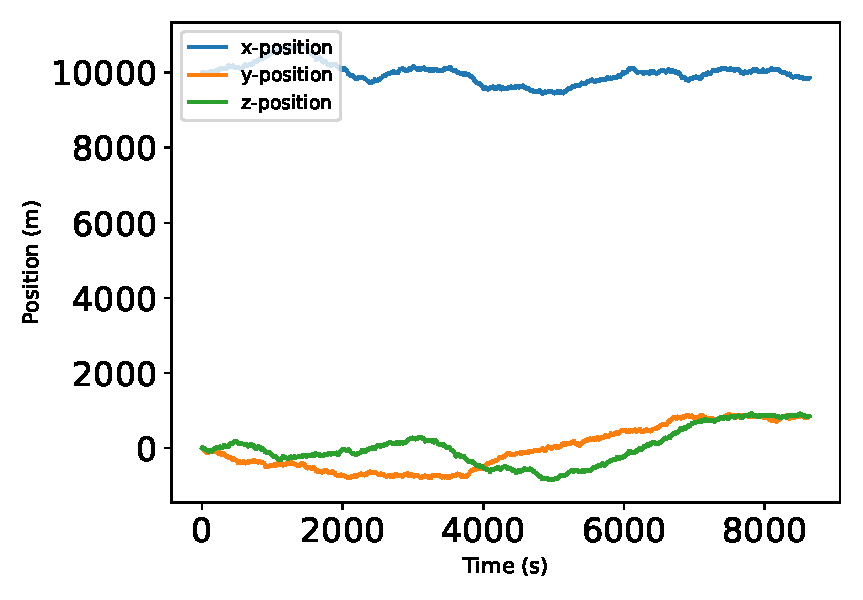
\includegraphics[height=0.4\textwidth, keepaspectratio]{AutoTeX/SimpleNavPos}}\caption{Simple Navigation Position Signal}\label{fig:SimpleNavPos}\end{figure}
\begin{figure}[htbp]\centerline{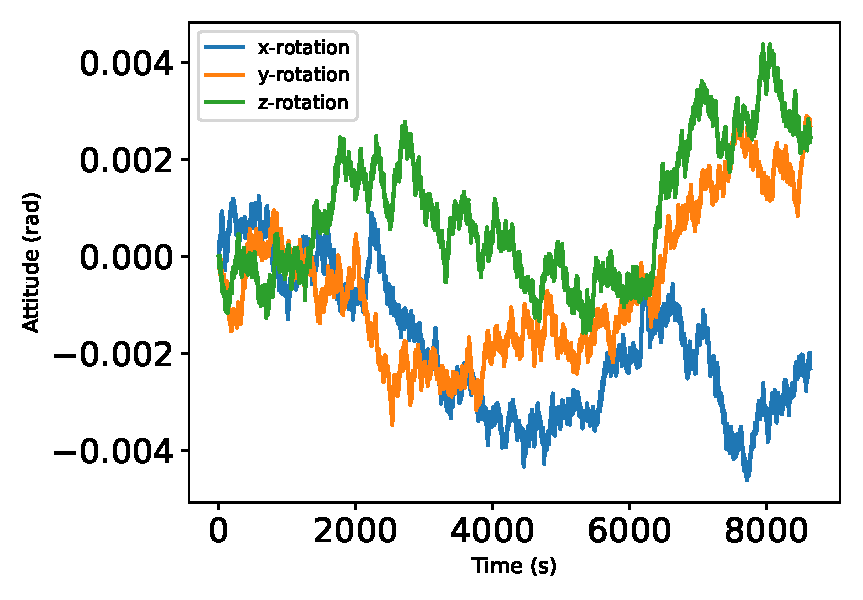
\includegraphics[height=0.4\textwidth, keepaspectratio]{AutoTeX/SimpleNavAtt}}\caption{Simple Navigation Att Signal}\label{fig:SimpleNavAtt}\end{figure}

In this figure, the nominal position that the error was being distributed about
 was [10000.0, 0.0, 0.0] in meters and the error was bounded such that the 
absolute value of the error was less than 1000 m.  The random walk had a white 
noise standard deviation of 5 meters.

In the model, the vehicle position, velocity, attitude, attitude rate, 
accumulated delta-velocity, and sun-pointing vector have errors applied 
separately.  Arguably the sun-pointing vector should just use the vehicle 
attitude and the Sun position to get is pointing accuracy, but the Sun can be 
sensed independently of this and that is why there is a separate error source
used for it.

The top-level model relies on a lower-level utility module called GaussMarkov 
that supplies the random walk process that is added to the truth states.  
Since the simpleNav model exercises this utility completely, the unit test 
documented here was also used to test the GaussMarkov model both in terms of 
functionality and in terms of code coverage.  The coverage results are included 
in a table in the results.